\documentclass[12pt, letterpaper]{article}
\usepackage{blindtext}
\usepackage{multicol}
\usepackage{listings}
\usepackage{graphicx}
\usepackage{wrapfig}
\usepackage{float}
\graphicspath{ {./images/} }
\title{Secure speedup of the future}
\author{Aitor Ruiz Garcia}
\date{September 2023}
\begin{document}
\maketitle
\begin{multicols}{2}
    \section{Abstract}
    JavaScript has emerged as a fundamental language in global development. Much of the success of Node.js, both in server-side applications and full-stack web applications (client-server), can be attributed to it.

    Node.js was primarily created to enable JavaScript to run on the server. The creator of Node never anticipated that JavaScript would be used for literally everything.

    JavaScript is employed in desktop applications using Electron, and in mobile applications using React Native or Ionic. As an interpreted language, it has a low entry barrier. As the default language of the web, it also boasts a wealth of interesting libraries.

    Node JS took the engine that runs JavaScript on Chrome, V8, and wrapped it in more C++ code to make it possible for it to interact with system calls.

    All these factors have contributed to the rise of JavaScript as the language of the future. Nonetheless, as the creator himself contends, it has experienced some 'growing pains'.
    \section{The problem}

    Ryan Dahl, the creator of Node.js, has expressed his regrets about the language. He has stated that he would not use JavaScript for a new project. He has also stated that he would not use Node.js for a new project. Node.js has grown past what it was intended to be, and it has become a 'monster'.

    Whyle experimenting with my TFG project, I have found some problems with the current state of the JavaScript ecosystem. I will explain them in the following sections. This TFM project was a web application with blockchain integrations for decentralized identity management. Even though this project is not in the scope of this TFM, it is important to understand the context of the problems that I have found.

    \subsection{No types}
    JavaScript, does not have a type checker. This means that the compiler does not check the types of the variables, and therefore, it is possible to assign a value of one type to a variable of another type. This can lead to unexpected errors in the code.

    Take a look at the following example:
    \begin{lstlisting}
    const user = {
        name = "",
        age = 0
    }

    console.log(user.email)
    \end{lstlisting}

    This small code will not rise any error to warn the developer that the user object does not have an email property. This lead to a runtime error, which is not good for the developer experience.

    It is even worse when the user recives the error in production, because the error will be shown to the user, and the user will not understand what is happening.

    This happens because JavaScript is a dynamic language, and it does not have a type checker.

    The original TFG used Next.js. A popular React-in-the-server framework. At the start of the project, I was not aware of the problems that I will explain in the following sections. I was using Next.js because it was the framework that I was more familiar with. Obviuslly, as the project grew, I started to have problems with the lack of types.

    \subsection{node\_modules}

    Node.js has a package manager called npm. This package manager is used to install libraries in the project. The problem is that the libraries are installed in the node\_modules folder, and this folder can grow a lot.

    By default npm does not softlinks the libraries between them. This means that if you have two libraries that use the same library, the library will be installed twice. More packages installed means more space used, and more time to install the packages. A CI build could take a lot of time to just install all the packages.

    \subsubsection{node\_modules security implications}

    As JavaScript is used in Web applications mainlly and both in the server and in the client, it is a good target to attack. Currentlly npm holds more that 1.6 millions packages.

    A sussesfull attack on a web framework would mean access a big chunk of browsers that a small porcentaje of them may be vulnerable.

    However the JavaScript in a browser is sandboxed, it is \textit{safer}. In Node.js this is not the case. All the code can interact with the file system and the whole internet.

    In the past there has been multiple cases of compromised npm, the most famous being \verb|colors| and \verb|faker.js|.

    The developer went rogue and introduced some infinite loops\dots

    Another notable example was \verb|UAParser.js|, and it downloaded and installed a password stealer and a cryptominer. It is important to note that this package was and still is used by millions of users daily.


    \subsection{Node GYP}

    Node GYP is the state of the art when creating native libraries in Node JS. This tool is originally from google. When google discontinuated it the comunity made a fork and the project continued.

    It is a tool writen in python, witch is not JavaScript, and it is inecessarilly complicated to write a native library.

    \section{The solution}

    Ryan Dahl, created Deno, a solution to his own issues created by working on Node JS without a clear plan.

    \subsection{TypeScript}

    TypeScript appeared in 2012 to add types to JavaScript. It works as a superset of JavaScript. Meaning all keywords would be valid in TypeScript but vicebersa.

    TypeScript does not work by changing V8, but making JavaScript the compile target of TypeScript. This allowed also targeting multiple versions of JavaScript and the use of polyfils if the desired API was not present.

    However TypeScript in this form, while very helpfull, it add more time to the development process because it now has to compile TypeScript to JavaScript and then run the intended program.

    Deno, translates TypeScript on the fly and feeds it to V8, meaning the whole process is just plug and play and developers do not have to configure an external tool, as \verb|tsc|, the compiler, can be pretty hard to set up and get it to behave.

    In the code, this mens that every variable would have an associated type and they could not change anywhere in the code.

    \begin{lstlisting}
    var name: string = "";
    \end{lstlisting}

    The variable name can not have another value asignated without being a string.

    \begin{lstlisting}
    name = 0;
    \end{lstlisting}

    This code will result in error as \verb|0| is not a string.

    This will catch multiple runtime errors.

    \subsection{URL based imports}

    A major change with Deno comes with the URL based imports the modules are cached and reused when needed.

    However with this as the script comes from an URL it may come with malicius code in it. How could a developer protect itself?

    \subsubsection{Security checks}

    Deno implements multiple checks to prevent uncontrolled access to the machine.

    \begin{itemize}
        \item //TODO: !!!!!
    \end{itemize}


    \subsection{Speedup}

    The solution that some projects owners have implemented to solve the performance is just using a compiled languague as a companion. This languagues \textit{in general} have better performance than interpreted ones.

    In the web space two projects stand out from the rest. The whole developer space arround the web development has grown exponentially and now more than ever a bundler is needed to combine all that information in a simple combination of HTML CSS and JS.

    \verb|SWC| and \verb|esbuild| are both tools that relly in other languagues to speedup. However this two project payed a big role in the development of this project.

    \subsubsection{SWC}

    SWC decided to compile a rust porgram and compile it into a binary. Then later they wrote some JS glue code to make it usable from a JS project.

    As this application is a pure CLI style application this approach is benefitial as it is only neccesary a small size of JS code. This is because they only need to pass the neccesary args to the rust binary and then the rust porgram takes over and packages the JS application.

    This can be benefitial in this objetive but a library that needs to run when the developer calls a function, the glue code must spawn a shell and that takes time. So much time that it may not be even be benefitial to use a native library.

    \subsubsection{esbuild}

    \verb|esbuild| decided to take another approach. They used wasm to create the library. As this project is writen in go, the whole go garbage collector has to be injected into the wasm code.

    This can result in larger install sizes and a bad developer experience as stated before.

    It's worth noting that wasm, even though it is an excelent tecnology and has brought very good speedup to the web, it still lacks a good memory management solution. This results in very good performance compared to JavaScript but not compared to the rest.

    \section{The code}

    The arrived solution is a dynamic library with a minimal TypeScript glue code.

    Deno offers an incredible dynamic library support with their native API.

    \begin{lstlisting}
    Deno.dlopen(
        test.lib,
        {},
    )
    \end{lstlisting}

    In this method the developer just has to locate the dll physically. It also needs to specify how the methods in the library work.
    The process wold be the following.

    \begin{enumerate}
        \item Peek at the file system to see if the dll is present. If the user did not allow from the launch flags Deno will ask for permision.
        \item Download the dll if the dll is not present. If the user did not allow from the launch flags Deno will ask for permision.
        \item Load the library and prepare it.
    \end{enumerate}

    \subsection{Speedy but memory safe}

    The final peace to this project is deciding how to secure the last part of the project. The obvious choice is a low lever languague that can really squeeze out the performance of the CPU.

    To prevent having some memory related issues some languagues have to be removed. Languagues like C and C++ the memory is managed my the developer and can result in segfaults and others.

    And if the focus is to have the best possible performance languagues with garbage colletion had to be rulled out.

    That only option left is \verb|Rust|.

    Rust uses a borrow checker to keep track of all the memory allocated while not allowing the allocation and deallocation by the user. That way it can garantee that all the memory that is needed will be used.

    If a variable is borrowed it means that it comes from another function and the current variable cannot be tranfered ownership. It means that the variable will continue living.

    If a variable is owned, when the function runs out of scope it will be dealocated.

    \begin{lstlisting}
        const a = 10:
        fun(a);
        foo(a);
    \end{lstlisting}

    In this code only the first function call will comply with the compiler. The other one will fail.

    In order for this code to work it will need to be changed.

    \begin{lstlisting}
        const a = 10;
        fun(&a);
        foo(a);
    \end{lstlisting}

    As the first function does not take ownership of the variable \verb|a| it does not get freed at the end, and can be user in the next function call.

    \subsubsection{Creating a dynamic library}

    In rust everything is just a compilation target so here it can just be specified that a library is wanted.

    There are multiple types of libraries, but the focus of this project is that this library can be used in other projects.

    \subsection{Where WASM fits}

    WASM, as mentioned before it is pretty usefull in the browser, where it belongs. Right now it is a bit early and the WASM API within the browser is still joung and the WASI libc library works but it is not there yet.

    \subsection{The data}

    Lets take a look to the actual data to see if this idea actually holds up. This tests have been conducted using strings from a collection of 36 characters repeated 1000 times to the same collection of 36 characters repeated to 2000 times. Each set is repeated 15 times and the average is calculated to rule out any errors.

    The data is collected one next to another. Meaning that no async functions are used an the deno and rust functions are runned one after the other, to rule out any OS induced noise.

    \subsubsection{Hardware used}

    This tests have been runned in a broad collection of hardware, all of the \verb|x86_64|.

    \begin{itemize}
        \item Github actions builders 2-core CPU \verb|x86_64|
        \item i9-12900H
        \item i5-1135G7
    \end{itemize}

    The data presented in this document will come from the CPU \textbf{i9-12900H}, however there is data present in the github repository that can be extracted from every commit added to the repo.

    In every test runned the results are the same but with obvious speed difference as the hardware selected are very diverse.

    \subsubsection{Hashing}

    The first part of the library to analize is hashing. The algorithm used to hash is bcrypt.

    //TODO: Entrar a fondo

    \begin{figure}[H]
        \centering
        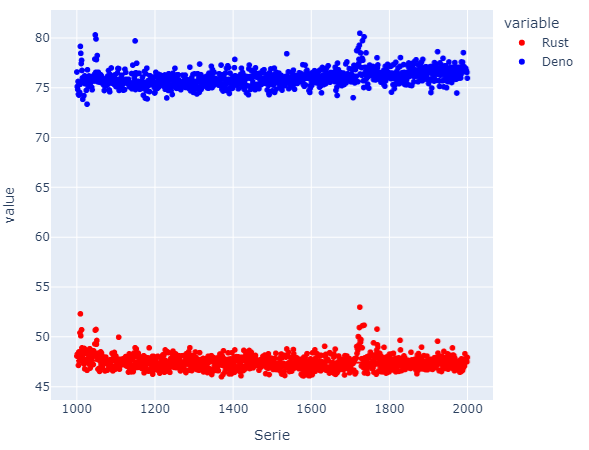
\includegraphics[width=0.45\textwidth]{hashing_lines}
    \end{figure}

    In this image it can be seen the creation of 1000 hashes and its cost in milliseconds with a bycrypt cost of 14. On average Rust is faster by 57\%.

    The trends here are not clear but it is aparent that the following 2 graphs.

    \begin{figure}[H]
        \centering
        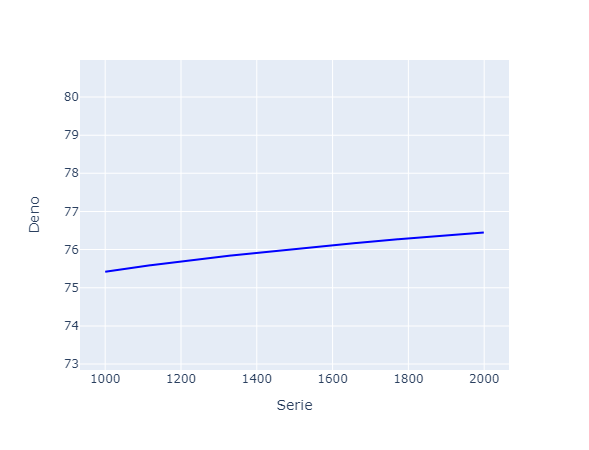
\includegraphics[width=0.45\textwidth]{trend_hash_deno}
    \end{figure}

    \begin{figure}[H]
        \centering
        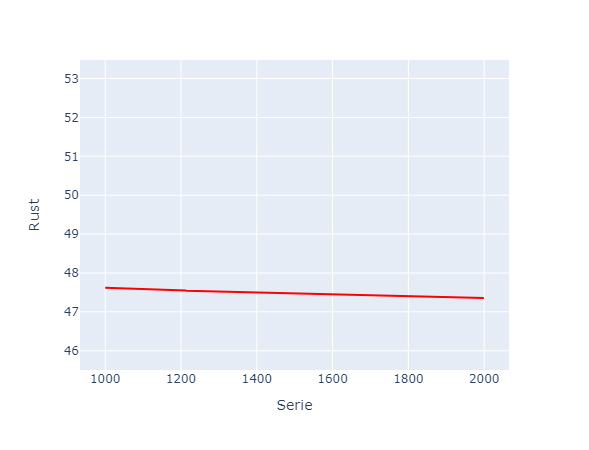
\includegraphics[width=0.45\textwidth]{images/trend_hash_rust.png}
    \end{figure}

    From the data some aspects can be deduced.
    \begin{itemize}
        \item The cost of hashing will go up faster than rust does.
        \item Rust will be more stable and grow less.
    \end{itemize}

    \subsubsection{Secret boxes}

    Secret boxes are a concept introduced by the library NaCl. A secret box is just a box with just one lock. This is just a metaphor for syncronous cryptography. The algorithm that will be used in this project. To be exact it will be used a variant called tweetnacl, witch is a library that manages to copy the exact functionality but fit in 100 tweets.

    The focus of this library is speed and a small footprint in the developer/user hard drive.

    \begin{figure}[H]
        \centering
        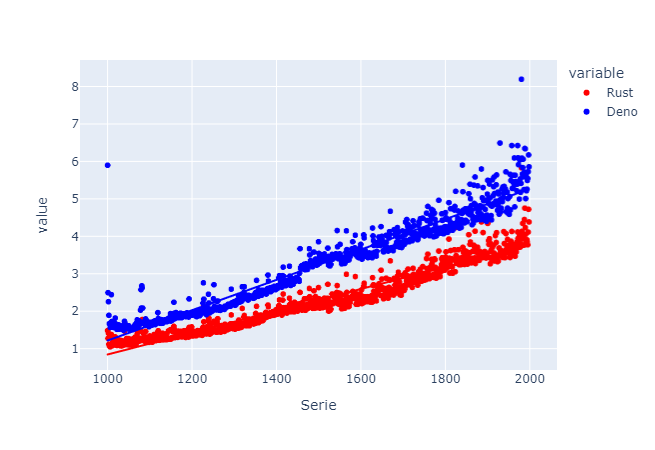
\includegraphics[width=0.45\textwidth]{images/secretbox_lines}
    \end{figure}

    In the graph there are some deno results that shotout from the predicted results. As this results do not appear in the rust variant they must come from variations on V8 function \textit{heat}. In V8 when a function is called it gets \textit{heat}. This means that it gets cached for later use and if a function gets executed a lot it gets stored in machine code, to maximize the performance.

    In this example again it can be seen that JavaScript is more unstable than Rust and will grow more.

    \begin{figure}[H]
        \centering
        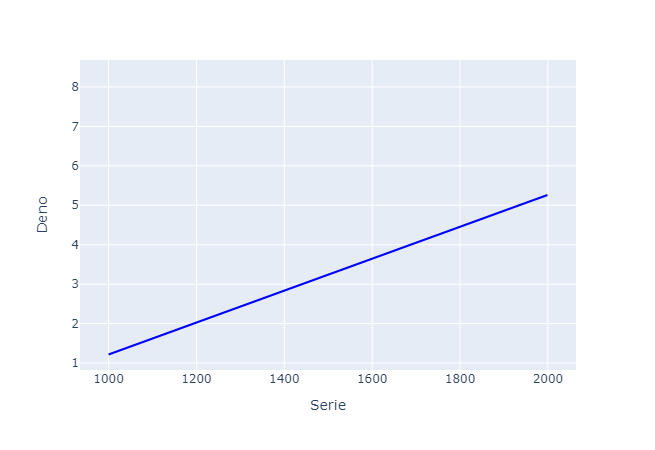
\includegraphics[width=0.45\textwidth]{trend_secretbox_deno}
    \end{figure}

    \begin{figure}[H]
        \centering
        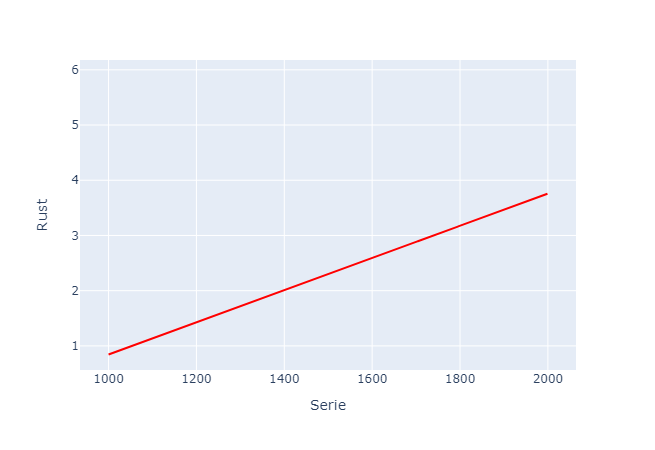
\includegraphics[width=0.45\textwidth]{images/trend_secretbox_rust}
    \end{figure}

    From the data some aspects can be deduced.
    \begin{itemize}
        \item The cost of encrypting will go up faster than rust does.
        \item Rust will be more stable and grow less.
    \end{itemize}

    \subsubsection{Box}

    A box is just a a container with two locks. Another metaphor for asymetric encryption. As the last algorithm, this is based in tweetnacl.

    \begin{figure}[H]
        \centering
        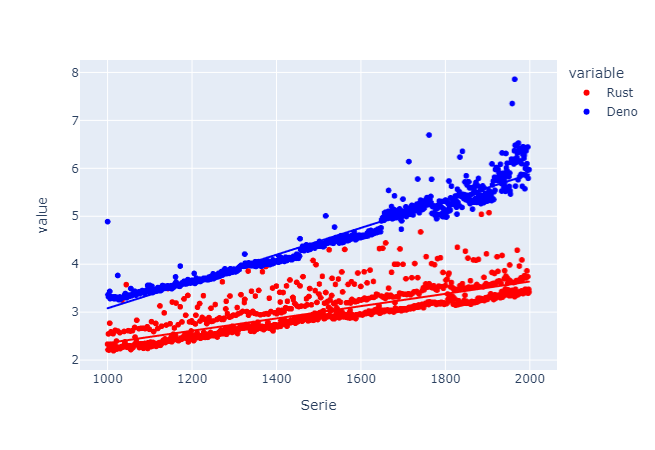
\includegraphics[width=0.45\textwidth]{images/box_lines}
    \end{figure}

    In this final algorithm, rust, while being more disperse it outperforms deno by a lot.

    \begin{figure}[H]
        \centering
        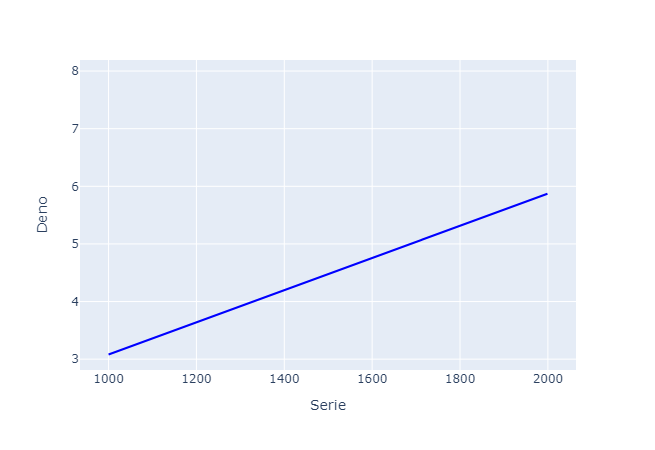
\includegraphics[width=0.45\textwidth]{trend_box_deno}
    \end{figure}

    \begin{figure}[H]
        \centering
        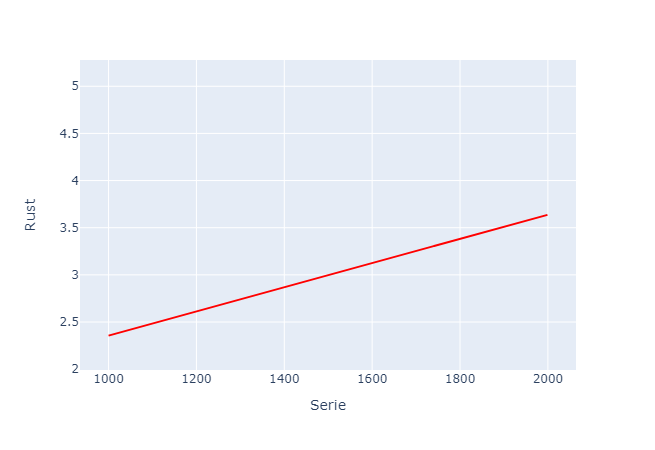
\includegraphics[width=0.45\textwidth]{images/trend_box_rust}
    \end{figure}

    From the data some aspects can be deduced.
    \begin{itemize}
        \item The cost of encrypting will go up faster than rust does.
        \item Rust will be more stable and grow less.
    \end{itemize}

    \section{Conclusions}



\end{multicols}
\end{document}